\documentclass[
aspectratio=169 % comment for 4:3
]{beamer}
\usepackage{tabularx}

\newcommand{\cmd}[1]{\texttt{\textbf{#1}}}
\newcommand{\args}[1]{\texttt{\textit{#1}}}

\usetheme[
hidetotal, % hide the total number of slides on the bottom right
hidenumbers, % hide current slide number
% hidename, % hide author name and title in footline
hidebullets, % use empty bullets in itemize
hidefootline, % hide the footline
%
% the previous options allow for a minimalistic style as recommended by Patrick
% Winston in his "how to speak" lecture at MIT
%
% sidebar, % show sidebar
hugetitle, % print main title in huge font
% thin, % use a thinner font
% bold, % use bold titles
% standardtitle, % use standard title slide (no picture)
]{mfrancois}

\setsecondarylogo{title/isia-logo} % Add a secondary logo to the title slide, optional
\settitleimage{title/raspberry} % Change the title slide image, optional (use images with a ratio identical to the one provided)

\author[F. Marelli]{François Marelli}
\affiliation[UMONS]{UMONS, ISIA Lab}
\title{Atelier Créactifs: Raspberry Pi}
\subtitle{Séance 7: Réseaux}
\extras{
\includegraphics[height=25pt]{title/creactifs}}
\date{30 mars 2026}

\graphicspath{{images}}

\begin{document}

\maketitle

\begin{frame}{Le protocole IP}{Internet Protocol}
    Pourquoi échanger des informations entre machines?

    \begin{itemize}
        \item Communiquer à distance (e.g. SSH)
        \item Offrir des services (e.g. Jellyfin)
        \item Partager des ressources (e.g. caméra RTSP)
    \end{itemize}

    \bigskip
    Comment ça marche? Avec le \alert{protocole IP} (Internet
    protocol)
    \begin{itemize}
        \item Adressage: identification des appareils
        \item Routage: acheminement des messages
    \end{itemize}

    \bigskip
    \(\rightarrow\) IP est à la base d'internet, omniprésent!
\end{frame}

\begin{frame}
    \centering
    \huge\alert{Envoyer des messages à distance:\\avant internet}
\end{frame}

\begin{frame}{Le routeur}{Le cœur du réseau}
    \begin{columns}
        \begin{column}{.45\textwidth}
            \centering
            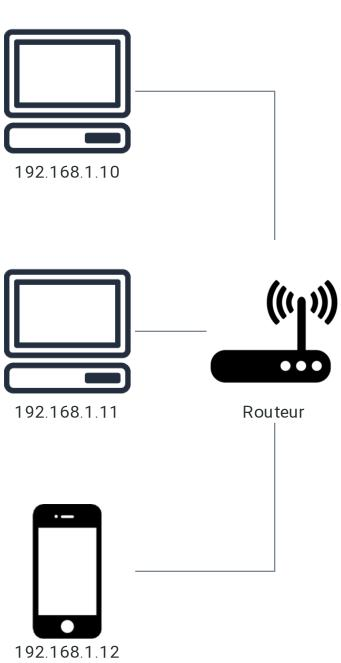
\includegraphics[height=0.75\textheight]{simple}
        \end{column}
        \begin{column}{.55\textwidth}
            Le routeur = \alert{le facteur}
            \begin{itemize}
                \item Connecte les clients
                \item Gère les adresses
                \item Transmet les messages
            \end{itemize}

            \bigskip
            \bigskip
            Exemples: Wi-Fi, câble

            \bigskip
            \bigskip
            Adresse IP (v4): 4 octets (0-255)
        \end{column}
    \end{columns}
\end{frame}

\begin{frame}{Les réseaux privés}{Isolation et extension}

    2 problèmes avec "chacun son adresse IP":
    \begin{itemize}
        \item Pénurie d'adresses IP (IPv4)
        \item Danger d'intrusion
    \end{itemize}

    \bigskip
    Solution: réseau privé
    \begin{itemize}
        \item Adresses privées (e.g. 192.168.1.x) valables localement
        \item Inaccessible depuis l'extérieur
    \end{itemize}

    \bigskip
    \bigskip
    Comment communiquer avec l'extérieur?
\end{frame}

\begin{frame}{Interface privé-public}{NAT: Network Address Translation}
    \begin{columns}
        \begin{column}{.5\textwidth}
            \centering
            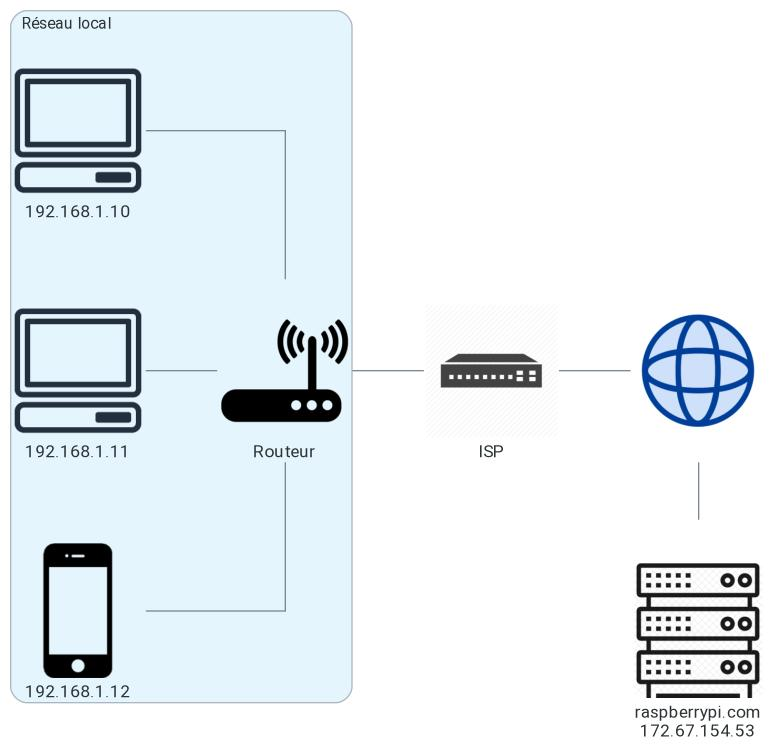
\includegraphics[height=0.75\textheight]{private}
        \end{column}
        \begin{column}{.5\textwidth}
            NAT = \alert{le secrétariat}
            \begin{itemize}
                \item Remplace les adresses privées par son adresse publique
                \item Redirige les réponses vers le bon client
            \end{itemize}

            \bigskip
            Ne marche que pour des \alert{requêtes sortantes}

        \end{column}
    \end{columns}
\end{frame}

\begin{frame}{Vue d'ensemble}{Plusieurs réseaux privés}
    \centering
    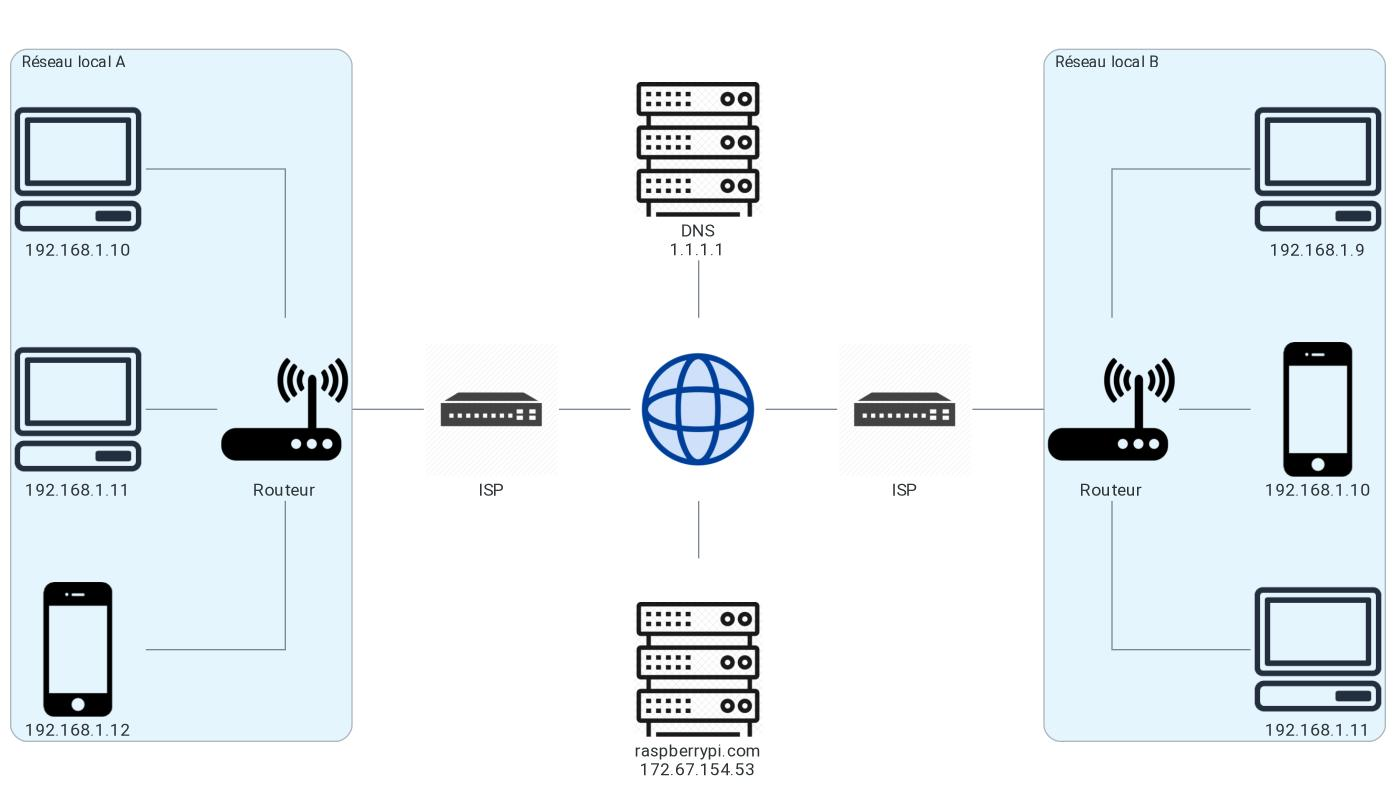
\includegraphics[height=.75\textheight]{network}
\end{frame}

\begin{frame}{Les réseaux virtuels}{Confidentialité et flexibilité}
    VPN (Virtual Private Network): renvoie les messages depuis son adresse
    \begin{itemize}
        \item Camouflage d'adresse IP
        \item Accès externe à un réseau privé
    \end{itemize}

    \bigskip
    \bigskip
    Plusieurs solutions de serveur VPN:
    \begin{itemize}
        \item OpenVPN (standard établi)
        \item WireGuard (moderne et performant)
    \end{itemize}

\end{frame}

\begin{frame}{Vue d'ensemble}{Avec un VPN}
    \centering
    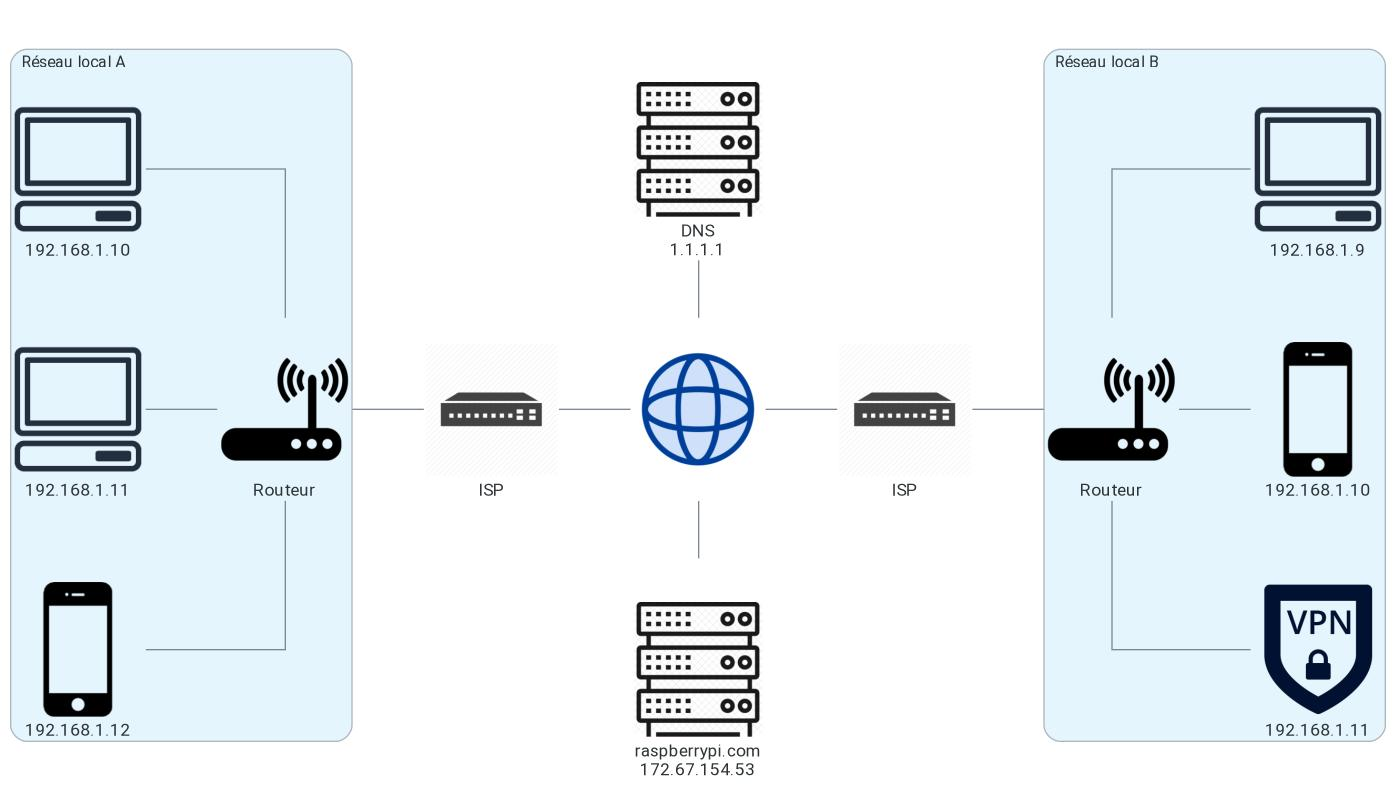
\includegraphics[height=.75\textheight]{vpn}
\end{frame}

\begin{frame}{Les réseaux virtuels maillés}{}
    Inconvénients du serveur VPN classique:
    \begin{itemize}
        \item Installation complexe à impossible dans un réseau privé
        \item Goulot d'étranglement pour le débit
    \end{itemize}

    \bigskip
    Solution: réseau maillé (mesh)
    \begin{itemize}
        \item Chaque appareil communique directement avec les autres
        \item Un serveur public met les clients privés en contact
        \item Agit comme un nouveau réseau privé virtuel
    \end{itemize}

    \bigskip
    Solutions: Tailscale, ZeroTier, \alert{NetBird}
\end{frame}

\begin{frame}{NetBird}{Solution de réseau maillé}
    Avantages:
    \begin{itemize}
        \item Open source
        \item Basé sur WireGuard
        \item Facile à installer et à utiliser
        \item Option gratuite généreuse
        \item Possibilité d'héberger son propre serveur
    \end{itemize}

    \bigskip
    \bigskip
    \url{https://netbird.io/}
\end{frame}

\begin{frame}[fragile]{Installation et lancement de NetBird}
    \begin{enumerate}
        \item Télecharger et installer NetBird
              \begin{verbatim}
curl -fsSL https://pkgs.netbird.io/install.sh | sh \end{verbatim}
              \medskip
        \item Lancer NetBird et se connecter
              \begin{verbatim}
netbird up \end{verbatim}

              Utilisateur: \texttt{rpi.creactifs@alumni.umons.ac.be}

              Mot de passe: \texttt{creactifsRPI26}
              \medskip
        \item Vérifier la connexion (quelle est votre adresse IP virtuelle?)
              \begin{verbatim}
netbird status
ip a
\end{verbatim}
    \end{enumerate}
    \bigskip

    Exercice: connectez-vous en SSH depuis un autre réseau

\end{frame}

\begin{frame}{Les noms de domaine}{DNS: Domain Name System}
    En pratique, on n'utilise pas directement les adresses IP

    \bigskip
    DNS = \alert{le botin téléphonique}
    \begin{itemize}
        \item Traduit les noms de domaine (e.g. raspberrypi.com) en adresses IP
        \item Toute communication débute par une requête DNS
    \end{itemize}

    \bigskip
    Options pour un serveur DNS:
    \begin{itemize}
        \item public (e.g. Google, Cloudflare)
        \item local (e.g. routeur UMONS)
        \item privé (e.g. sur un Raspberry Pi)
    \end{itemize}
\end{frame}

\begin{frame}{Vue d'ensemble}{Cheminement d'une page web}
    \centering
    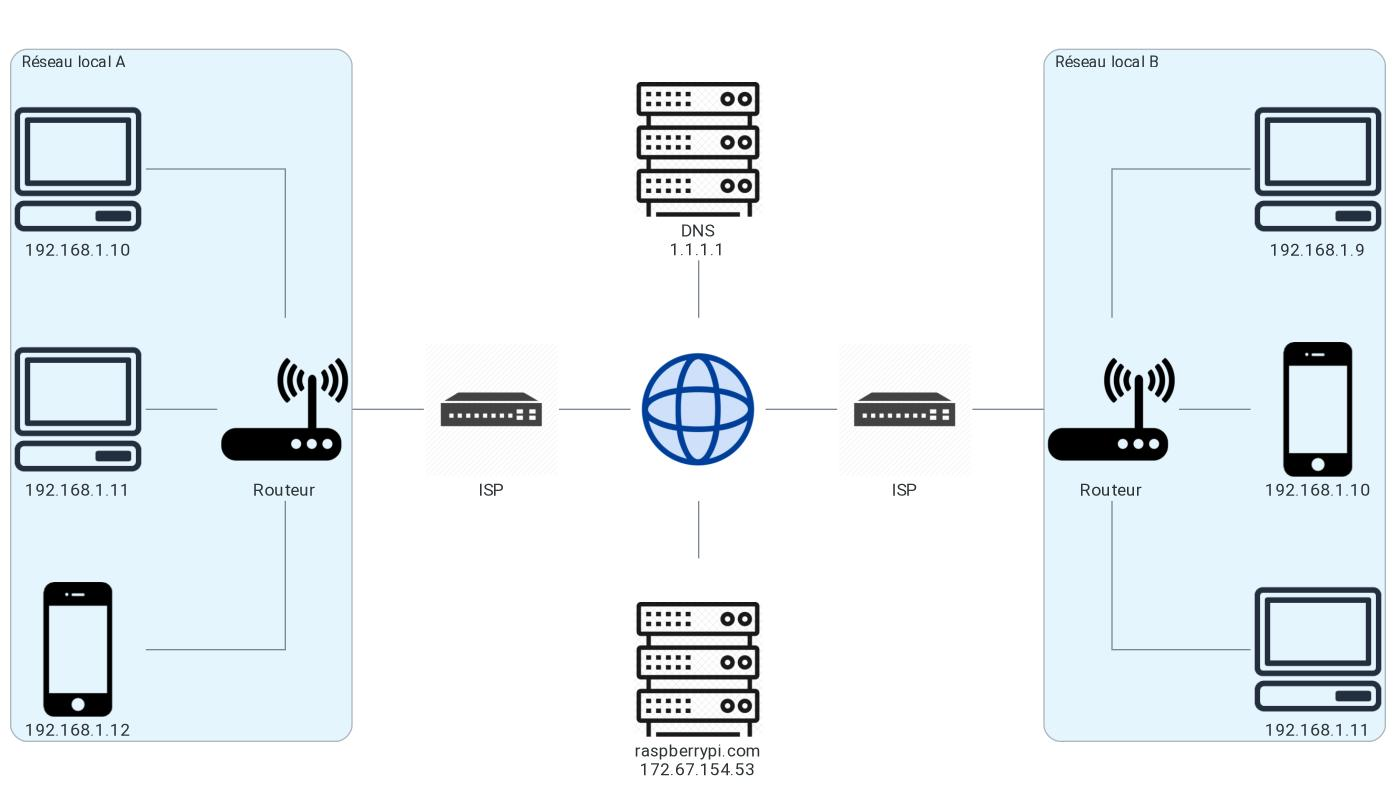
\includegraphics[height=.75\textheight]{network}
\end{frame}

\begin{frame}{Le bloquage de pubs}
    Bloquer les pubs au niveau du DNS:
    \begin{itemize}
        \item Serveur DNS privé
        \item Liste de domaines à bloquer
    \end{itemize}

    \medskip
    \(\rightarrow\) les requêtes vers des pages publicitaires sont bloquées

    \bigskip
    \begin{itemize}
        \item[+] bloquage de pubs pour tous appareils
        \item[+] bande passante réduite (pubs non chargées)
        \item[+] protection de la vie privée (moins de tracking)
        \item[-] impossible de bloquer les pubs "sur-site" (e.g. YouTube)
    \end{itemize}

    \bigskip
    \alert{Attention}: si mal configuré, un serveur DNS peut vous empêcher
    d'accéder à internet!

\end{frame}

\begin{frame}{Pi-hole}{Bloquage de pubs pour Raspberry Pi}
    \begin{columns}
        \begin{column}{.2\textwidth}
            \centering
            
\includegraphics[width=.9\textwidth]{pihole}
        \end{column}
        \begin{column}{.8\textwidth}

            Pi-hole: solution de serveur DNS privé pour Raspberry Pi
            \begin{itemize}
                \item Open source
                \item Utilisation simple (web)
                \item Bien documenté
            \end{itemize}

            \bigskip
            \url{https://pi-hole.net/}

        \end{column}
    \end{columns}

\end{frame}

\begin{frame}[fragile]{Pi-hole}{Installation et configuration}
    \begin{enumerate}
        \item Télécharger et lancer le script d'installation:
              \begin{verbatim}
curl -sSL https://install.pi-hole.net | bash \end{verbatim}

        \item Suivre les étapes du script, en choisissant les options par
              défaut\\(ne pas se préoccuper de la configuration IP)
        \item Accéder à l'interface web avec l'adresse et le mot de passe
              fournis par le script
        \item Configurer la connexion internet pour utiliser Pi-hole comme
              serveur DNS\\(utiliser 127.0.0.1)
    \end{enumerate}

    \bigskip
    \bigskip
    En situation réelle, il faut configurer son routeur pour que tout le réseau
    utilise Pi-hole

    \(\rightarrow\) aussi possible via NetBird!
\end{frame}

\begin{frame}{Validation de la configuration}
    \cmd{nslookup}\args{ nom.de.domaine}: envoyer et afficher une requête DNS

    \bigskip
    Installation:
    \cmd{sudo apt}\args{ install dnsutils}

    \bigskip
    Tester la configuration:
    \cmd{nslookup}\args{ raspberrypi.com}

    \(\rightarrow\) quelle est l'adresse du serveur DNS?
\end{frame}

\end{document}
